\documentclass[UTF8]{article}
\usepackage{ctex}
\usepackage{ulem}
\usepackage{amssymb}
\usepackage{amsmath}
\usepackage{graphicx}
\newtheorem{thm}{定义}[section]
\newtheorem{notation}[thm]{记号}
\newtheorem{lemma}[thm]{引理}

\makeatletter
\newcommand{\rmnum}[1]{\romannumeral #1}
\newcommand{\Rmnum}[1]{\expandafter\@slowromancap\romannumeral #1@}
\makeatother

\title{8 定义\\Definitions\\[2ex]\begin{large}读书笔记\end{large}}
\author{许博}
\date{}

\begin{document}
\maketitle
	\section{定义的本质(nature)}
	\noindent
	在逻辑和数学课本中,定义是必要的。因此我们将为$\lambda{\rm C}$添加含有定义的扩展,得到的推导系统记为$\lambda{\rm D}$,将在第十章中描述。而一个简单的前身记为$\lambda{\rm D_0}$,将在第九章中描述。本章将讨论定义的本质特征,以及如何形式化它们。
	
		引入定义的主要原因是为了表示并突出(highlight)有用的概念。逻辑和数学都基于某些概念,其中大部分都是其它概念的复合。通过给它们指定名称来挑选值得注意的概念非常方便。
		
		如“一个矩形是一个有四个直角的四边形”,值得注意的概念是“一个有四个直角的四边形”,而我们给它指定名称“矩形”。其中“四边形”以及“直角”的解释假定已经在之前给出。
		
		引入的名字不仅可以使用自然语言中的单词,也可以新发明单词或者符号,比如 c 或 $D_n$。而像 c 或$D_n$多半用于临时使用,但它们和更永久(permanent)的名字(如“矩形”)没有本质区别。所有名字的一个重要特征就是可以使重复引用了这些名字关联的对象或概念的表述更加紧凑。引入定义的一个更实际的原因是:如果没有定义,逻辑或数学的文本会迅速增长而超过合理的范围。
		
		还有一种引入新名字的情况是引入变量,如“令 x 为一个实数,Let x be a real number”,两者的区别在于变量作为一个集合中任意一个实体的名字,而定义的名字则作为一个确定是东西或概念的名字。
	
	\section{归纳和递归定义}
	\noindent
	在我们的类型理论中,没有归纳定义或者归纳类型用以基本(primitive)构造。在有些类型理论中定义自然数的类型,归纳地由常数 0 和后继函数构建,自动地生成了归纳证明原则以及通过有根据的递归定义函数的可能性。
	
		归纳定义可以在更高阶的逻辑中被定义为谓词,或者作为公理假设。
		
		至于递归定义,目的是通过一个算法描述某个对象。比如自然数$n$的阶乘$n!$可以通过递归结构描述:
		
		$fac(0) = 1$,
		
		$fac(n+1)=fac(n)*(n+1)$
		
		我认为,归纳和递归的差异在于归纳由 base case 衍生出集合中所有的成员,而递归是求某一个成员的算法(或过程),其中复用自身。
		
		在本书的后面将展现我们可以利用描述符$\iota$而不使用递归定义来完成,其中$\iota$给一个唯一存在的实体一个名字。通过不包括递归定义,我们达到了两个目标:
		
		\noindent
		- 保持系统相对简单
		
		\noindent
		- 避免引入递归定义带来的复杂性,比如需要表明每个递归定义表示一个对每个输入都有唯一结果的可终止算法
		
		一个显而易见的缺陷是,类似$fac$的函数不是一个程序,因此也不能被执行。作为后果,$fac(3)=6$需要一个证明。
		
	\section{定义的格式}
	\noindent
	我们从数学中引用如下用于定义的标准格式:
		
		$a:=\mathcal{E}$
		
		表示$a$被定义为$\mathcal{E}$,则$a$是给$\mathcal{E}$的名字,$\mathcal{E}$是一个描述值得被命名或记住的概念的表达式。
		
		\begin{thm}(Definiendum, defined name, defined constant, definiens)
			
			- 在$a:=\mathcal{E}$中,名字$a$被称作$definiendum$(被定义的东西,the thing to be defined),也被称作$defined name$或$defined constant$
			
			- 表达式$\mathcal{E}$是$definiens$,即“定义的东西,the thing that defines”或“确定了含义是什么的表达式”。
		\end{thm}
	
		我的理解是$definiendum$是被下定义的项,而$definiens$是下定义的项所定义的东西,因此 the thing that defines 中的 that 指代了 the thing to be defined。
		
		对于其它更复杂的定义,需要一些“环境,setting”,通过作为上下文形式化。为了便于阅读,参数列表会跟随定义,比如“递增,increasing”需要从集合$\mathbb{R}$到集合$\mathbb{R}$的函数$f$,通过在上下文中引入$\mathbb{R}$和$f:\mathbb{R}\rightarrow\mathbb{R}$,然后以$increasing(f) := ...$表示。尽管其中的参数列表可以省略,但为了便于阅读不予省略(除非参数列表为空)。
		
	\section{定义的实例化}
	\noindent
	将定义中的参数替换为具体的变量或良构的表达式,称为(参数的)实例化。如$increasing(f)$中$f$以$\lambda x:\mathcal{R}.x^3$实例化。当然,实例化需要满足上下文中要求的类型。
	
		在定义给出之后,实例化定义时,环境上下文不需要再给出,同时定义可以在脱离定义的上下文中直接使用,但仍需要保证对应参数的类型满足要求。
		
		常量的两个不同方面(引入和使用)蕴含了一个常量具有两个不同的生命阶段:\\
		(1) “出生,birth”,当在定义中引入时\\
		(2) “生命之路,path of life”,当在不同的情况下使用时,通过对于参数的不同实例化
		
		我认为便于定义的参数实例化,也是参数列表跟随定义的一个重要原因。
		
	\section{用于定义的形式化格式}
	\noindent
	之前所提到的定义具有如下形式:
	
		$\Gamma\triangleright a(x_1,...,x_n):=\mathcal{E}$
		
		其中$\Gamma$是一个上下文,$a$是一个后缀参数列表的常量(definiendum),被定义为$\mathcal{E}$(definiens)。引入符号$\triangleright$作为上下文和剩余部分的分隔符。因此这个表达式的含义为:
		
		在上下文$\Gamma$中,我们定义$a(x_1,...,x_n)$为$\mathcal{E}$。
		
		因为我们工作在一个类型化的环境中,需要为 definiens 添加类型,也同样是 definiendum 的类型,因此格式变为:
		
		$\Gamma\triangleright a(x_1,...,x_n):=M:N$,\\
		其中 M 是 definiens 而 N 是它的类型,同样也是$a(x_1,...,x_n)$的类型。
		
		参数列表$(x_1,...,x_n)$包含了上下文中的主体变量,因此一个定义形如:
		
		$x_1:A_1,...,x_n:A_n\triangleright a(x_1,...,x_n):=M:N$。
		
		其中$n$是一个自然数,所以可为 0 (如果$\Gamma$为空上下文)。后文中使用一个缩写的表示用以通用格式:
		
		$\overline{x}:\overline{A}\triangleright a(\overline{x}):=M:N$
		
		在元语言(meta-language)中使用如下缩写:
		
		\begin{notation}(1) $\overline{x}$表示变量的列表$x_1,...,x_n$
			
			(2) $\overline{A}$表示表达式的列表$A_1,...,A_n$
			
			(3) $\overline{x}:\overline{A}$表示上下文$x_1:A_1,...,x_n:A_n$
		\end{notation}
	
	\section{依赖于假设的定义}
	\noindent
	存在定义依赖于假设,比如定义最小元素的时候,通常已经假设了给定集合在给定关系上是偏序的。此时在上下文中添加假设:
	
		\noindent
		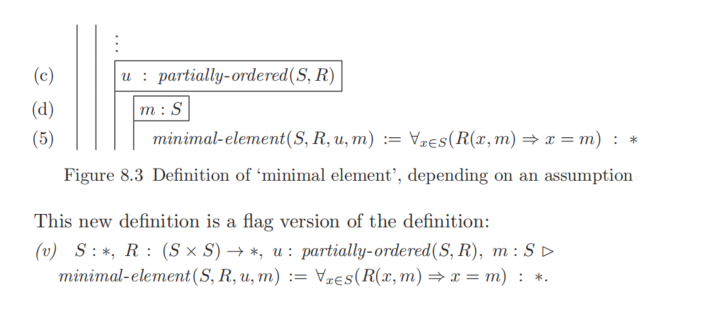
\includegraphics[width=0.93\linewidth]{"../imgs/8-1.png"}
	
	\section{给证明以名字}
	\noindent
	在之前给出的定义中,定义过以下常量:\\
	- 集合,类型为$*$;\\
	- 成员,类型为一个集合;\\
	- 命题,类型为$*$。
	
		其中定义成员,有如$c:=\cfrac{1+\sqrt{5}}{2}$,类似地,我们可以定义命题的证明。
		
		如:
		
		\noindent
		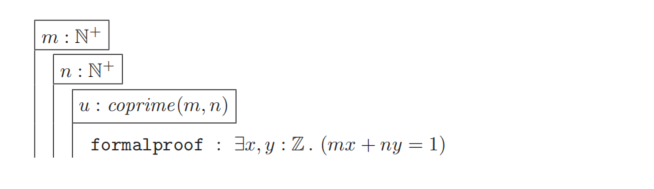
\includegraphics[width=0.93\linewidth]{"../imgs/8-2.png"}
		
		其中$\bf formalproof$是命题$\exists x,y:\mathbb{Z}.(mx+ny=1)$的一个证明,而其之前的声明$u:...$是一个假设,也即在此假设下,存在命题的一个证明,接下来我们可以给该证明一个名字:
		
		\noindent
		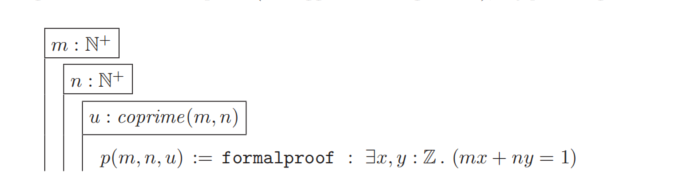
\includegraphics[width=0.93\linewidth]{"../imgs/8-3.png"}
		
		如此一来,在之后实例化时,证明可以直接复用。
\end{document}
